

\chapter{Methodology} \label{ch:methodology}
This chapter defines the methodology used to develop the framework for testing the \gls{db}. The chapter is divided into several sections, each focusing on a specific aspect of the methodology. The first section introduces the development process as a whole, including a detailed plan with measurable milestones to ensure a systematic and robust development. The  second section discusses the first milestone which describes the test setup, including \gls{cs}, \gls{sw} algorithm, and \gls{hil} system. The third section provides an overview of the \gls{ds} used for training and testing the model, including \gls{dc}, annotation, and preprocessing techniques. Furthermore it discusses the \gls{od} algorithm and its pipeline, including the selection of a pre-trained model and the training process. Finally, the fourth section covers integration techniques, including algorithm integration with \gls{cs} and synchronization with \gls{hil} system.

\section{Introduction}
The methodology used in this project is divided over 3 main milestones. The first milestone focuses on the test setup, which includes the selection of a suitable \gls{cs}, light control, and the integration of a \gls{hil} system. The goal of this milestone is to develop a complete closed loop setup that is ready to integrate the model and run the detection process in the test environment. The second milestone involves the preparation of a \gls{ds} in an automated way using photoshop files, perform annotations, preprocessing and augmentation to increase model generalization. Furthermore, the  milestone includes the training of the chosen \gls{od} model using the prepared \gls{ds} and testing its performance on camera pictures from the \gls{cs}. The third milestone focuses on the integration of the trained \gls{od} model with the \gls{sw} that synchronizes with the \gls{hil} system.

\section{Test Setup}
The test setup is a crucial part of the project as it provides the environment in which the \gls{db} will be tested and evaluated. The setup includes the selection of a suitable \gls{cs}, light control, and the integration of a \gls{hil} system. The goal of this milestone is to develop a complete closed loop setup that is ready to integrate the model and run the detection process in the test environment. The following sections provide an overview of the test setup, including the \gls{cs}, light control, and \gls{hil} integration.

\subsection{Light Control}
To ensures that the \gls{cs} captures images under a controlled optimum lighting conditions, a light control system is an essential part of the test setup. This is important for the performance of the \gls{od} model, as variations in lighting can significantly affect the quality of the detection model. The light control system should be capable of providing adjustable and uniform illumination across the entire \gls{fov} of the camera. Additionally, it should prevent any external light sources from interfering with the captured images, this is important to ensure that no glare or reflections are present in the images, which can lead to false detections or misclassifications.

KTM uses a light control system that consists of a box with aluminum frame and black walls to prevent any external light or light reflections. The box is equipped with a set of LED lights that can be adjusted to provide the desired level of illumination. The lights are positioned to ensure that the entire \gls{fov} of the camera is evenly illuminated, and they can be controlled remotely to adjust the brightness and color temperature as needed. This allows for complete control over the lighting conditions during the testing process, ensuring that the images captured by the camera are of high quality and suitable for the \gls{od} model. Figure \ref{LightControl} shows the light control system used in the test setup.

\begin{figure}[!htb]
    \centering
    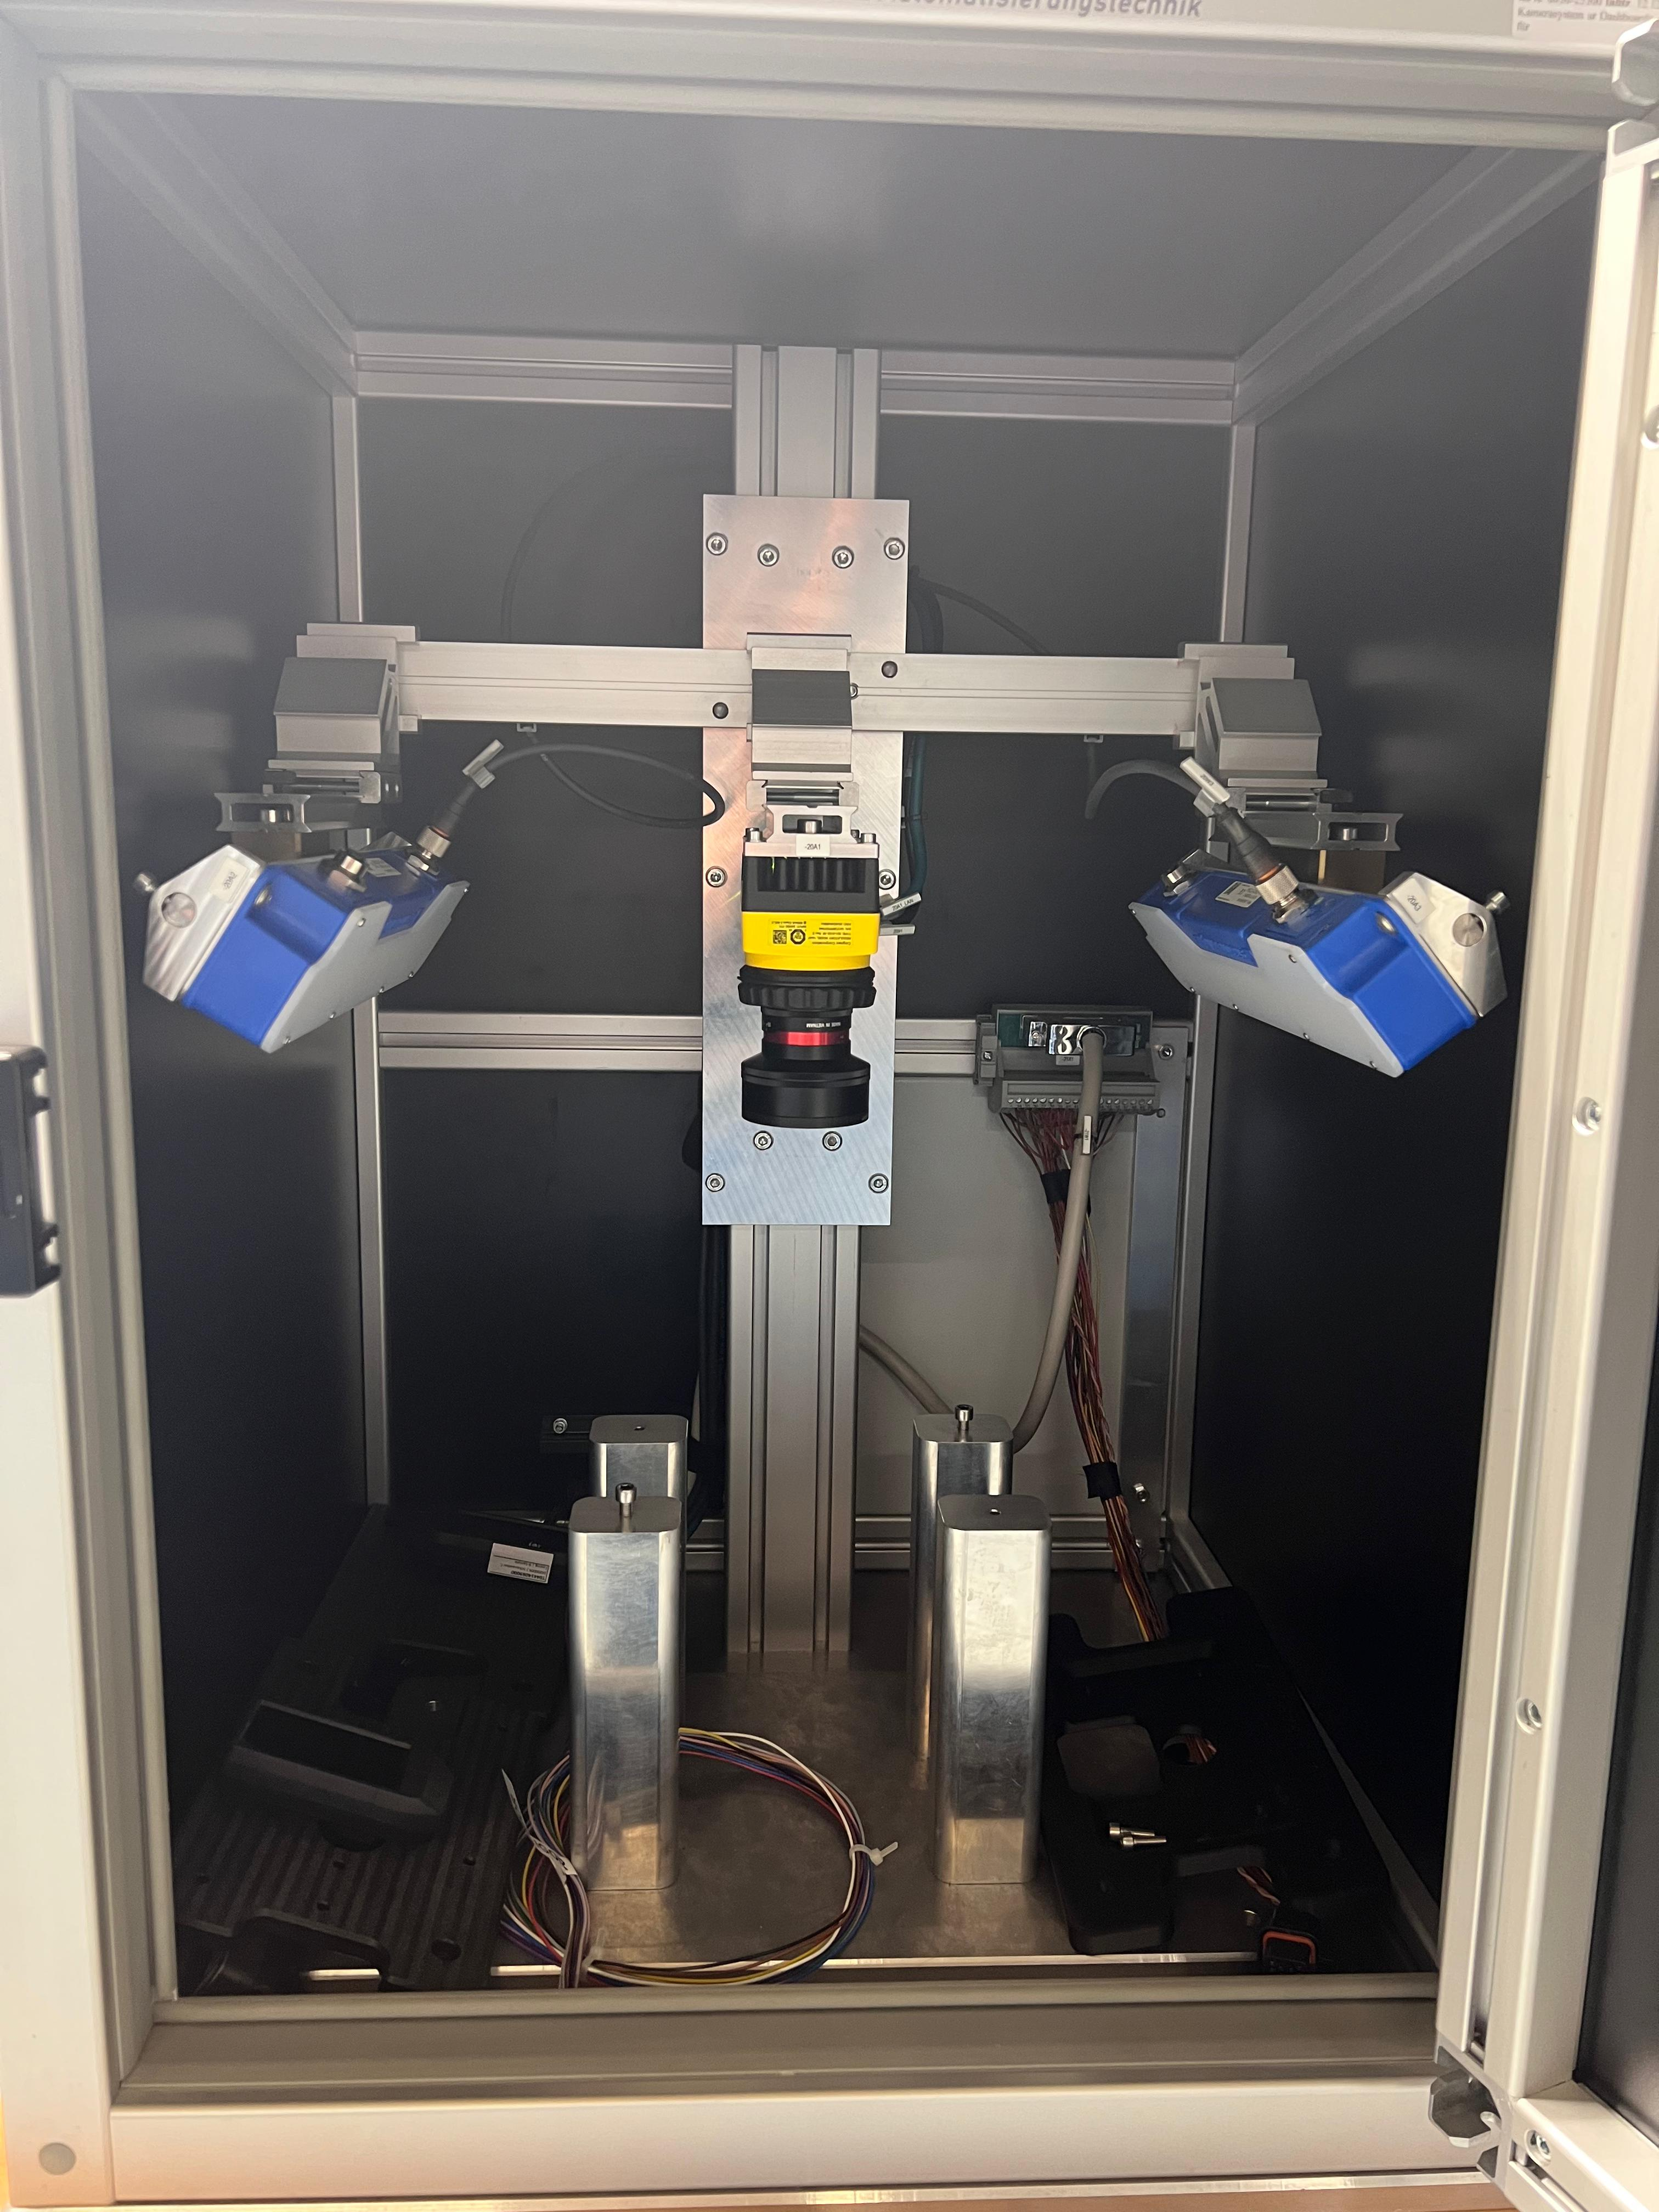
\includegraphics[width=0.6\textwidth]{Figures/Light_Control_Box.jpg}
    \caption{Light control system used in the test setup.}
    \label{LightControl}
\end{figure}

The box provides a mounting structure for the \gls{cs} to ensure that the \gls{cs} is positioned correctly and securely during the testing process. It also includes a mounting structure for the the \gls{db} to ensure that the distance between the \gls{cs} and the \gls{db} is consistent. Additionally, a cable inlet is provided to allow for the connection of the \gls{cs} and the \gls{db} without compromising the light control system.

Insert an image of the light control system with the camera and \gls{db} mounted inside the box.

\subsection{Camera System}
The \gls{cs} is an important component of the test setup as it captures images of the \gls{db} for testing and evaluation. It should be capable of capturing high-resolution images with a wide \gls{fov} to ensure that all relevant objects are included in the captured frames. Since a light control system is used, the \gls{cs} does not need to be highly sensitive to light variations and since the \gls{db} is a static object, the camera does not need to be highly sensitive to motion blur.

Due to the availability of a \gls{cs} at KTM , it was recommended to use the available \gls{cs}. The \gls{cs} used in this project is a high-resolution camera provided by Cognex, a company specialized in \gls{cs}s for industrial use cases. The camera is capable of capturing images at a resolution of up to 12 mega pixels (4096 x 3000) pixels, which is sufficient for the \gls{od} model to detect and classify objects accurately \cite{Cognex_Camera}. The camera provides a variety of communication interfaces, including Ethernet, which allows for easy integration with the \gls{sw} to capture and retrieve images smoothly through \gls{telnet} and \gls{ftp} protocols. Figure \ref{Cognex_Camera} shows the \gls{cs} used in the test setup.

\begin{figure}[!htb]
    \centering
    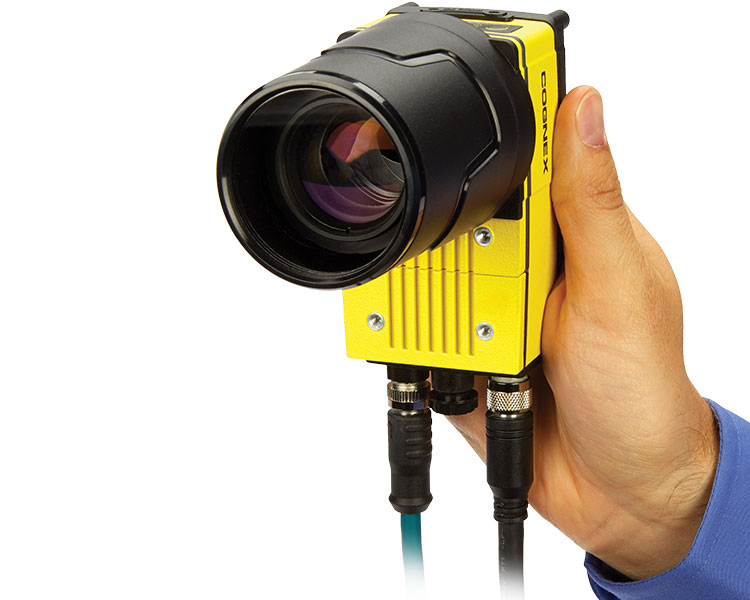
\includegraphics[width=0.5\textwidth]{Figures/In-Sight 9000 in hand.jpg}
    \caption{Cognex \gls{cs} used in the test setup \cite{Cognex_Camera}.}
    \label{Cognex_Camera}
\end{figure}

The camera is mounted inside the light control box to ensure that it is positioned correctly and securely during the testing process. The mounting structure allows for easy adjustment of the camera's position and angle to ensure that the entire \gls{db} is captured in the images. Additionally, the camera is connected to a computer via Ethernet, which allows for easy access to the captured images and integration with the \gls{sw}. Figure \ref{Camera_Mounting} shows the \gls{cs} mounted inside the light control box.

\begin{figure}[!htb]
    \centering
    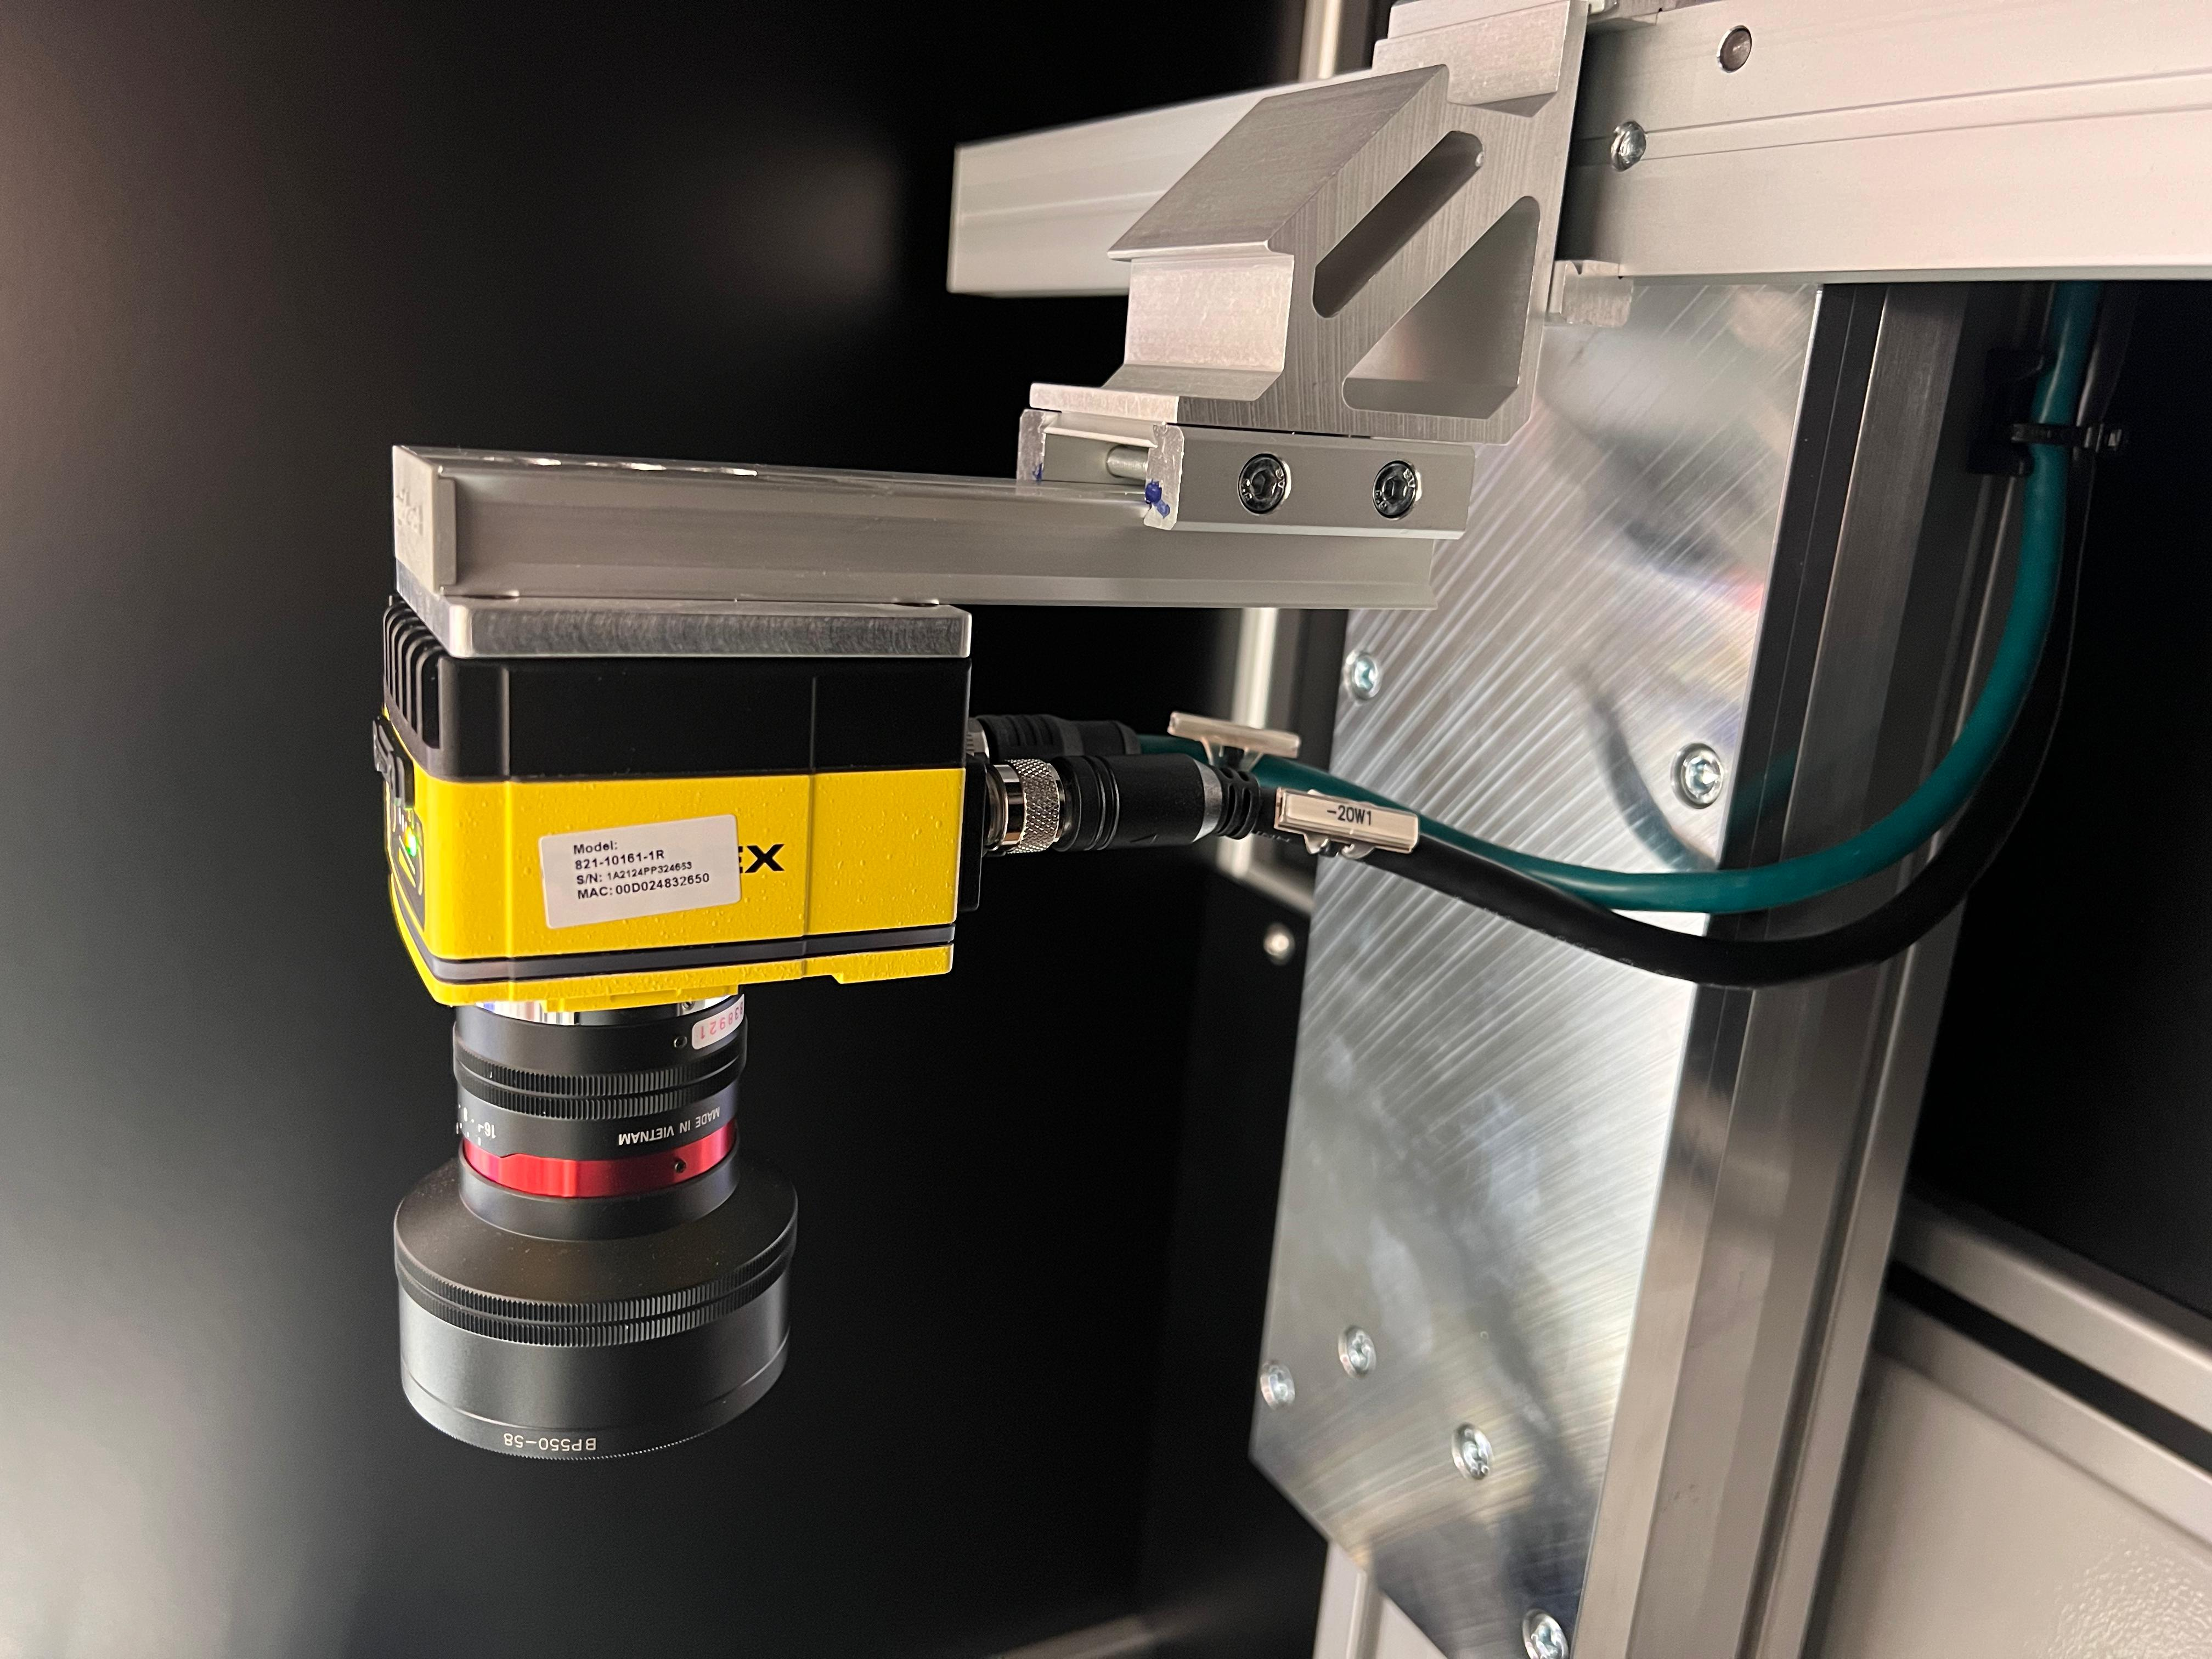
\includegraphics[width=0.6\textwidth]{Figures/Camera_Mounting.jpg}
    \caption{\gls{cs} mounted inside the light control box.}
    \label{Camera_Mounting}
\end{figure}

\subsection{Hardware In The Loop System}
The \gls{hil} is considered as the backbone of this test setup as it simulate the real-world environment in which the \gls{db} will operate. It allows for the testing and evaluation of the \gls{db} in a controlled environment. In this project, a Vector-provided \gls{hil} system is used, it is featuring a toolchain that includes Vector CANoe and VTest Studio, which are used to to create test scenarios and send the required CAN messages to the \gls{db} to trigger a specific frame.

Moreover, the toolchain uses .NET framework which allows for easy integration with the \gls{sw} algorithm to send requests from the \gls{hil} to the \gls{sw} to capture an image and process using the \gls{od} model then compare it with the expected results and a response is sent back to the \gls{hil} system. Based on this evaluation, the \gls{hil} system automatically logs the outcome of the test case as either passed or failed.

The communication between the \gls{hil} system and the \gls{sw} algorithm is done through a TCP/IP connection, which allows for real-time communication and synchronization between the two systems. This allows the \gls{sw} algorithm to capture images from the \gls{cs} and process them using the \gls{od} model, while the \gls{hil} system sends requests and receives responses in real-time.


\section{Object Detection And Classification Algorithm}
.........
\subsection{Overview Of Object Detection Pipeline}
.........
\subsection{Selection Of the Pretrained Model}
.........
\subsection{Data Preprocessing And Augmentation}
.........
\subsection{Model Fine-Tuning And Training Process}
..................
\subsection{Post-Processing And Object Classification}
.........
\subsection{Model Evaluation Metrics}
.........
.........
\section{Integration Techniques}
.........
\subsection{Algorithm Integration With Camera System}
.........
\subsection{Synchronization With Hardware In The Loop System}
.........
\subsection{Data Flow And Processing Pipeline}
.........
